\documentclass[tikz,border=12pt]{standalone}
\usepackage[T1]{fontenc}
\usepackage[utf8]{inputenc}
\usepackage{lmodern}
\usetikzlibrary{arrows.meta}

\definecolor{ink}{HTML}{25344A}
\definecolor{quebg}{HTML}{EEF2F8}
\definecolor{queborder}{HTML}{405B7B}
\definecolor{comobg}{HTML}{EAF6EE}
\definecolor{comoborder}{HTML}{34835A}

\tikzset{
  % Cartões voltaram ao tamanho original (2.38cm / 1.95cm): só a altura
  % da faixa de fundo muda nesta versão, não os cartões.
  card/.style={
    rectangle, rounded corners=4pt, fill=white,
    line width=0.8pt, text width=2.38cm,
    minimum height=1.95cm, align=center,
    inner xsep=5pt, inner ysep=5pt,
    font=\small\sffamily, text=ink
  },
  what/.style={card, draw=queborder!75},
  how/.style={card, draw=comoborder!80},
  relation/.style={
    -{Latex[length=2.5mm]},
    draw=ink!65, line width=0.9pt
  }
}

\begin{document}
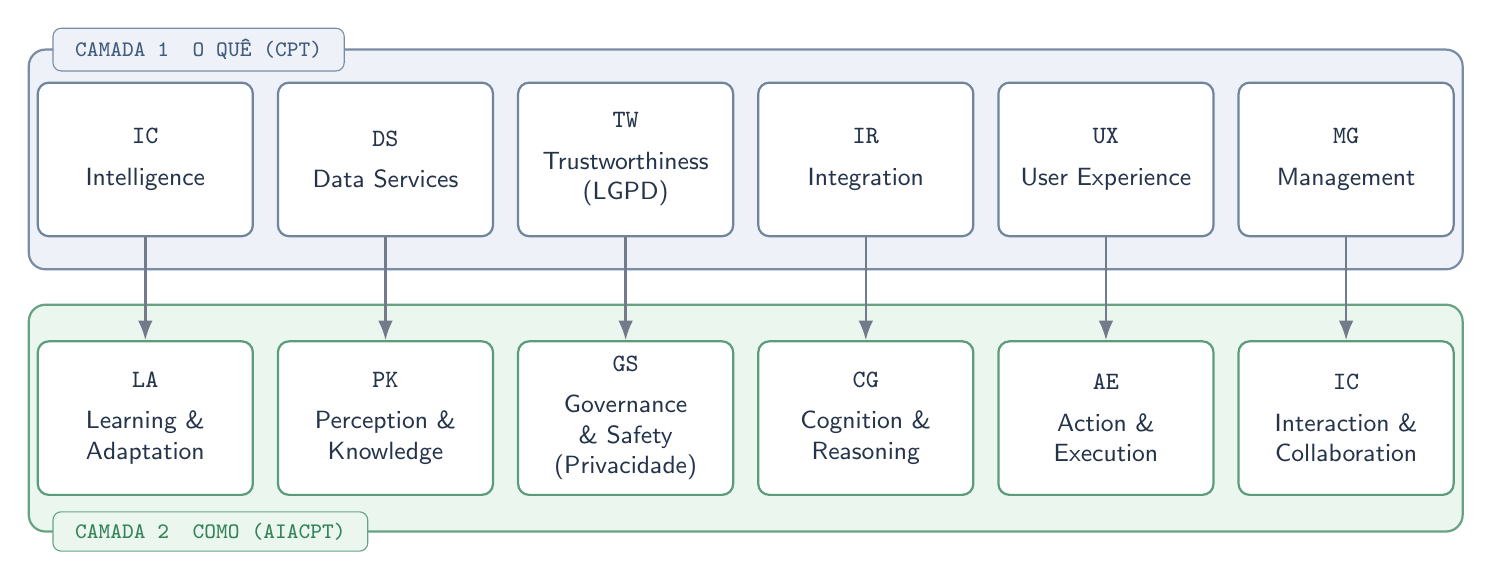
\begin{tikzpicture}[font=\sffamily]

  % \node[font=\bfseries\Large, text=ink] at (7.625,7.12)
    % {Arquitetura de capacidades do gêmeo digital};

  % ---- Faixas de fundo: altura -10% (como antes) + vão branco entre
  % elas reduzido para 50% do valor anterior (0.90 -> 0.45). Cada banda
  % desliza 0.225 em direção à outra, mantendo a própria altura e os
  % cartões no lugar.
  \filldraw[fill=quebg, draw=queborder!70,
            rounded corners=6pt, line width=0.8pt]
    (-1.48,2.865) rectangle (16.73,5.655);

  \filldraw[fill=comobg, draw=comoborder!75,
            rounded corners=6pt, line width=0.8pt]
    (-1.48,-0.465) rectangle (16.73,2.415);

  % Camada 1: aba na borda superior da faixa azul (y acompanha o novo topo).
  \node[
    anchor=west, fill=quebg, draw=queborder!70,
    rounded corners=3pt,
    inner xsep=8pt, inner ysep=4pt,
    font=\ttfamily\footnotesize, text=queborder
  ] at (-1.18,5.655)
    {\textbf{CAMADA 1}\quad O QUÊ (CPT)};

  % Camada 2: aba na borda inferior da faixa verde (y acompanha o novo fundo).
  \node[
    anchor=west, fill=comobg, draw=comoborder!75,
    rounded corners=3pt,
    inner xsep=8pt, inner ysep=4pt,
    font=\ttfamily\footnotesize, text=comoborder
  ] at (-1.18,-0.465)
    {\textbf{CAMADA 2}\quad COMO (AIACPT)};

  % ---- Cartões: recentralizados no meio de cada faixa (faixas ficam
  % fixas daqui pra frente). Banda 1 centro = (5.655+2.865)/2 = 4.260.
  % Banda 2 centro = (2.415-0.465)/2 = 0.975.
  \node[what] (q1) at (0,4.260)
    {{\bfseries\texttt{IC}}\\[4pt] Intelligence};
  \node[what] (q2) at (3.05,4.260)
    {{\bfseries\texttt{DS}}\\[4pt] Data Services};
  \node[what] (q3) at (6.10,4.260)
    {{\bfseries\texttt{TW}}\\[4pt] Trustworthiness\\(LGPD)};
  \node[what] (q4) at (9.15,4.260)
    {{\bfseries\texttt{IR}}\\[4pt] Integration};
  \node[what] (q5) at (12.20,4.260)
    {{\bfseries\texttt{UX}}\\[4pt] User Experience};
  \node[what] (q6) at (15.25,4.260)
    {{\bfseries\texttt{MG}}\\[4pt] Management};

  \node[how] (c1) at (0,0.975)
    {{\bfseries\texttt{LA}}\\[4pt] Learning \&\\Adaptation};
  \node[how] (c2) at (3.05,0.975)
    {{\bfseries\texttt{PK}}\\[4pt] Perception \&\\Knowledge};
  \node[how] (c3) at (6.10,0.975)
    {{\bfseries\texttt{GS}}\\[4pt] Governance \& Safety\\(Privacidade)};
  \node[how] (c4) at (9.15,0.975)
    {{\bfseries\texttt{CG}}\\[4pt] Cognition \&\\Reasoning};
  \node[how] (c5) at (12.20,0.975)
    {{\bfseries\texttt{AE}}\\[4pt] Action \&\\Execution};
  \node[how] (c6) at (15.25,0.975)
    {{\bfseries\texttt{IC}}\\[4pt] Interaction \&\\Collaboration};

  \foreach \i in {1,...,6}
    \draw[relation] (q\i.south) -- (c\i.north);

\end{tikzpicture}
\end{document}